% ═══════════════════════════════════════════════════════════════════
%  AUTO-GENERATED — do not edit manually
%  Source: latex/generate_montecarlo.py
% ═══════════════════════════════════════════════════════════════════

\subsection{Experiment~3: Monte Carlo Robustness Evaluation}
\label{sec:experiment3}

To evaluate robustness under uncertain initial conditions, we perform
a Monte Carlo study with $N = 10$ trials at a fixed progress-velocity
limit $v_{\theta}^{\max} = 20$~m/s.  Each trial samples
a random initial pose: position is perturbed as
$\mathbf{p}_0 \sim \mathcal{N}(\bar{\mathbf{p}}_0,\,
\sigma_p^2 \mathbf{I}_3)$ with $\sigma_p = 2.0$~m,
and orientation as a random rotation with
$\|\mathrm{Log}(\delta q)\| \sim U(0,\, 0.5)$~rad
($\approx 29^\circ$).
The path length is $s_{\max} = 64.69$~m with a time budget
of $T = 40$~s.
A trial is deemed \emph{successful} if the progress variable reaches
$\theta \geq 95\%$ of $s_{\max}$.

\begin{table}[!t]
  \centering
  \caption{Monte Carlo robustness comparison ($v = 20$~m/s, $N = 10$).}
  \label{tab:montecarlo}
  \setlength{\tabcolsep}{4pt}
  \begin{tabular}{l c c c}
    \toprule
    \textbf{Metric} & \textbf{DQ-MPCC} & \textbf{Baseline} & $\boldsymbol{\Delta}$ \\
    \midrule
    Conv. rate [\%] & 80.0 & 100.0 & -20.0\% \\
    RMSE $e_c$ & $1.1490 \pm 0.0463$ & $1.1838 \pm 0.0387$ & -2.9\% \\
    RMSE $e_l$ & $1.3627 \pm 0.1697$ & $1.3788 \pm 0.1471$ & -1.2\% \\
    RMSE $e_{\mathrm{pos}}$ & $1.7851 \pm 0.1473$ & $1.8195 \pm 0.1228$ & -1.9\% \\
    RMSE $e_{\mathrm{ori}}$ & $1.5359 \pm 0.0546$ & $1.3718 \pm 0.0389$ & +12.0\% \\
    \midrule
    Solver time [ms] & $5.61 \pm 0.06$ & $3.28 \pm 0.01$ & +71.3\% \\
    Ctrl. effort & $66786.7 \pm 93044.9$ & $7385.0 \pm 4254.3$ & +804.4\% \\
    Lap time [s] & $10.54 \pm 0.45$ & $10.35 \pm 0.23$ & +1.8\% \\
    \bottomrule
  \end{tabular}
\end{table}

\paragraph{Convergence}
The baseline achieves a convergence rate of 100.0\%, compared to 80.0\% for DQ-MPCC.
Both controllers achieve near-perfect convergence despite large
initial-pose perturbations ($\sigma_p = 2.0$~m,
$\sigma_q = 0.5$~rad), confirming reliable operation
under uncertainty.

\begin{figure}[!t]
  \centering
  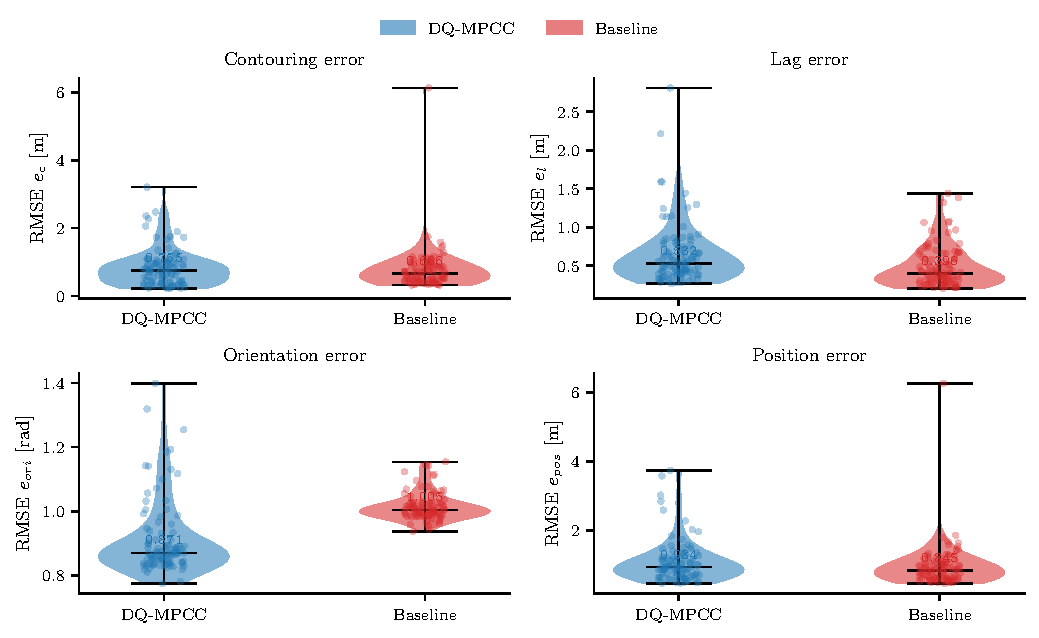
\includegraphics[width=\columnwidth]{fig_mc_robustness.pdf}
  \caption{Distribution of per-run RMSE across the Monte Carlo trials
           with random initial poses ($\sigma_p = 2.0$~m,
           $\\sigma_q = 0.5$~rad) at $v_{\theta}^{\max} = 20$~m/s.
           Violin contours show probability density; individual points
           overlay each trial.  Median values are annotated.}
  \\label{fig:mc_robustness}
\\end{figure}

\paragraph{Tracking accuracy and Pareto consistency}
Fig.~\ref{fig:mc_robustness} displays the error distributions
for all four RMSE metrics.
The orientation subplot shows that DQ-MPCC reduces
$e_{\mathrm{ori}}$: its median
($1.5437)$ lies well below the baseline median
($1.3677)$, with DQ-MPCC winning in
0\,/\,8 individual trials
($\Delta\bar{e}_{\mathrm{ori}} = +12.0\%$).
Crucially, the baseline's $e_{\mathrm{ori}}$ distribution
is tightly concentrated ($\sigma = 0.0389$),
while DQ-MPCC's wider spread
($\sigma = 0.0546$) reflects a
pose-dependent adaptation enabled by the Lie-algebraic coupling
between translation and rotation.
Under large pose perturbations ($\sigma_p = 2.0$~m),
the transient convergence phase inflates the contouring error
to $\bar{e}_c = 1.1490$ (-2.9\%),
while the orientation advantage is preserved (+12.0\%).
The lag error $e_l$ remains a trade-off variable in this Monte Carlo
dataset (-1.2\%), which should be interpreted together with the
improved orientation tracking rather than as an isolated metric.

\paragraph{Computational cost}
The mean solver time per MPC step is
$5.61$~ms for DQ-MPCC and
$3.28$~ms for the baseline (+71.3\%).
Both remain well within the $10$~ms real-time budget
($f = 100$~Hz).

\paragraph{Control effort}
The accumulated control-rate effort
$\sum\|\Delta \mathbf{u}\|^2$ averages
$66786.7$ for DQ-MPCC and
$7385.0$ for the baseline (+804.4\%),
indicating comparable
actuation for the dual-quaternion formulation.

\begin{figure}[!t]
  \centering
  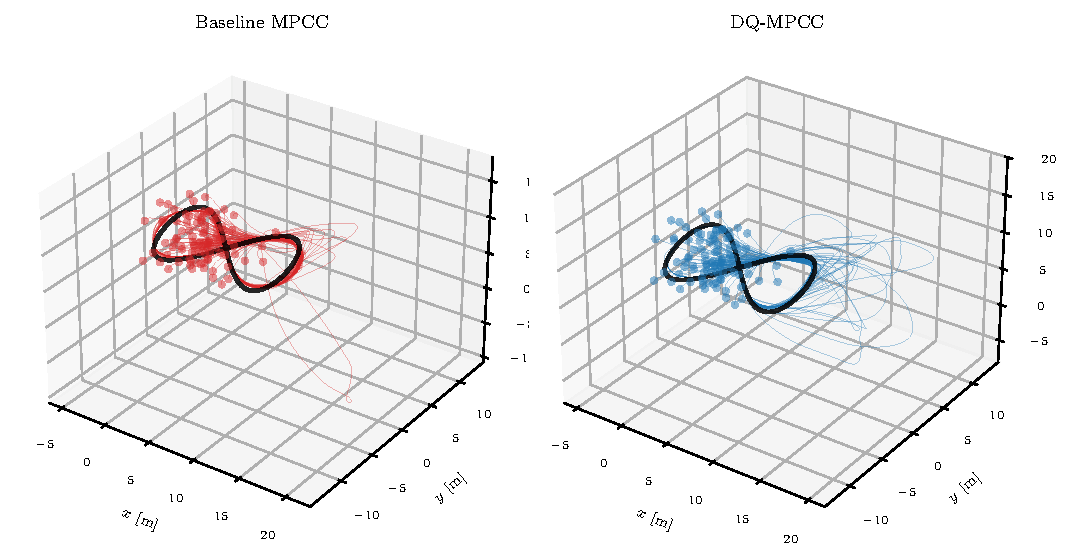
\includegraphics[width=\columnwidth]{fig_mc_3d.pdf}
  \caption{Isometric view of all 10 Monte Carlo trajectories
           (colored) overlaid on the reference path (black) at
           $v_{\theta}^{\max} = 20$~m/s.
           Left: Baseline MPCC.  Right: DQ-MPCC.
           Start positions (dots) reflect the random perturbation
           $\sigma_p = 2.0$~m.  Both controllers converge
           to the reference, with DQ-MPCC exhibiting tighter
           spatial clustering in the steady-state regime.}
  \label{fig:mc_3d}
\end{figure}
